\section{TTL y MOS, entradas abiertas y compatibilidad entre tecnolog\'ias}

\subsection{Compuertas discretas con entrada desconectada}

\subsubsection{Descripci\'on general}
En la Fig. \ref{fig:open_gate_circuits} se muestra el esquema general bajo an\'alisis, se utiliza una compuerta AND de tecnolog\'ia TTL,
particularmente 74LS08 y una compuerta OR de tecnolog\'ia CMOS particularmente 74HC32. El objetivo es estudiar y comparar el comportamiento
cuando se deja una de las entradas sin un estado definido, obteniendo conclusiones sobre ello.

En el proceso de medici\'on se buscar\'a observar la entrada y salida de cada circuito, con la entrada al aire, o un estado bajo o alto y analizando
la susceptibilidad del mismo a fuentes de ruido externas o de interferencia. Se parte de la hip\'otesis de que el estado sin definir hace al circuito vulnerable
frente al ruido, y existen argumentos f\'isicos para sospechar que habr\'a mayor influencia en uno de los casos.

\begin{figure}[H]
    \centering
    \begin{tabular}{c c}
        \includegraphics[scale=0.8]{../EJ5/Recursos/ttl_open.png} &
        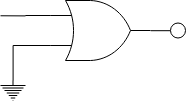
\includegraphics[scale=0.8]{../EJ5/Recursos/cmos_open.png}
    \end{tabular}
    \caption{Compuerta AND de tecnolog\'ia TTL y OR de tecnolog\'ia CMOS}
    \label{fig:open_gate_circuits}
\end{figure}

\subsubsection{Resultados}
En las Figs. \ref{fig:cmos_or_al_aire} y \ref{fig:ttl_and_al_aire} se observan los resultados de las mediciones, las cuales ordenadas de arriba hacia abajo y de izquierda a derecha, corresponden a la medici\'on
con entrada en estado bajo, en estado alto, con entrada al aire y luego con la mano apoyada. Para todos los casos la se\~nal amarilla corresponde a la entrada de la compuerta y la verde la salida.

Vale mencionar, que en los casos de estado bajo donde el valor promedio medido por el osciloscopio da negativo, se observ\'o con volt\'imetro digital que el valor era aproximadamente nulo y se atribuye
a defectos de la resoluci\'on digital del osciloscopio el asignar a tal magnitud un valor de dicho signo.

\begin{figure}[H]
    \centering
    \begin{tabular}{c c}
        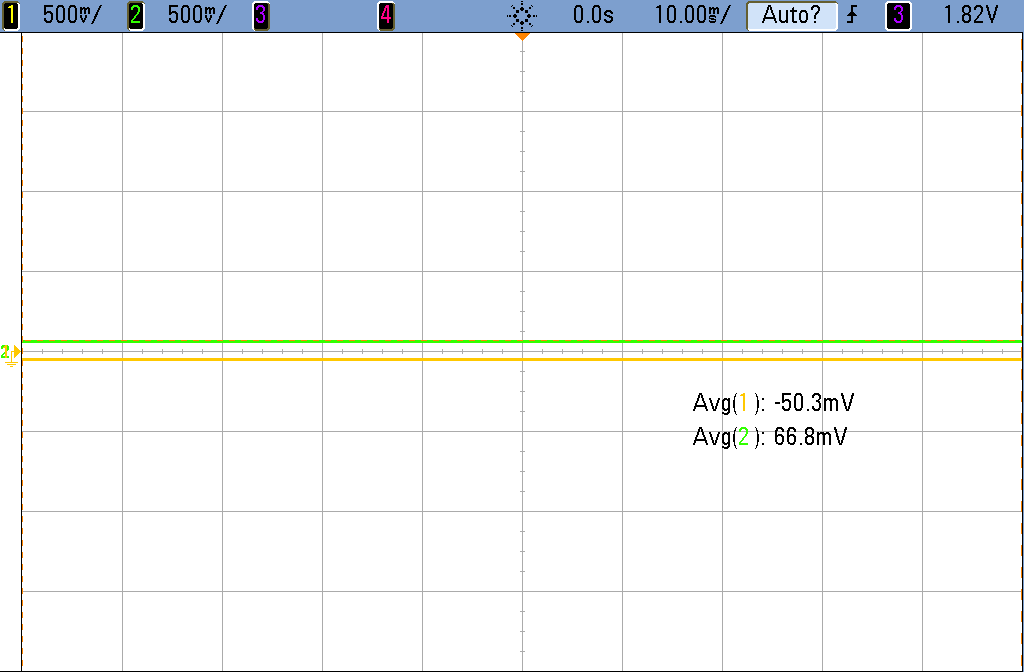
\includegraphics[scale=0.2]{../EJ5/Mediciones/Osciloscopio/CMOS_OR_SOLA/cropped_entrada_estado_bajo.png} &
        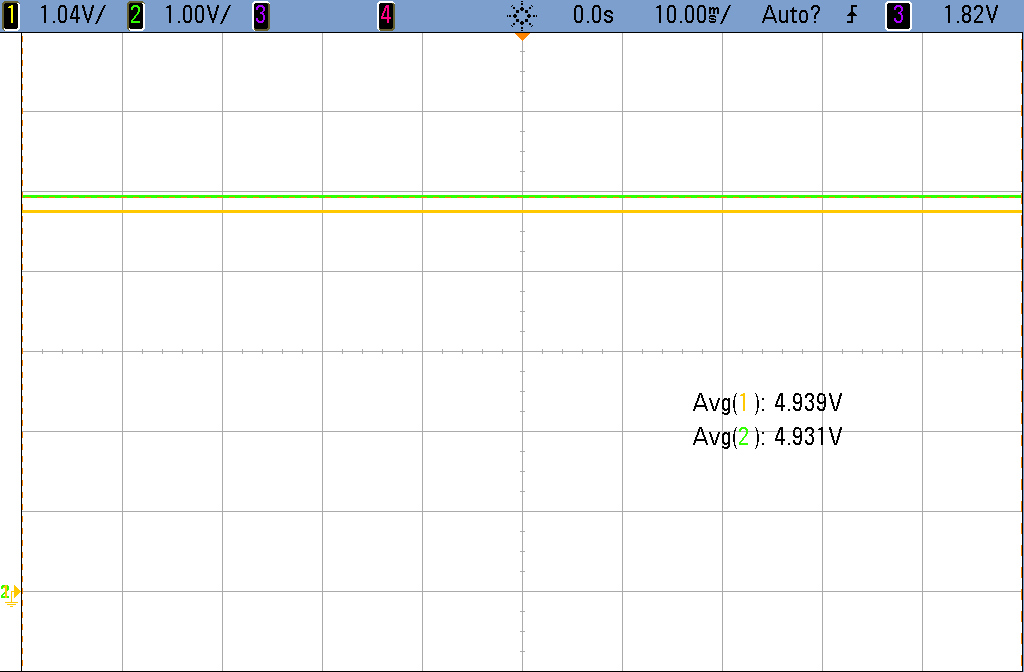
\includegraphics[scale=0.2]{../EJ5/Mediciones/Osciloscopio/CMOS_OR_SOLA/cropped_entrada_estado_alto.png} \\
        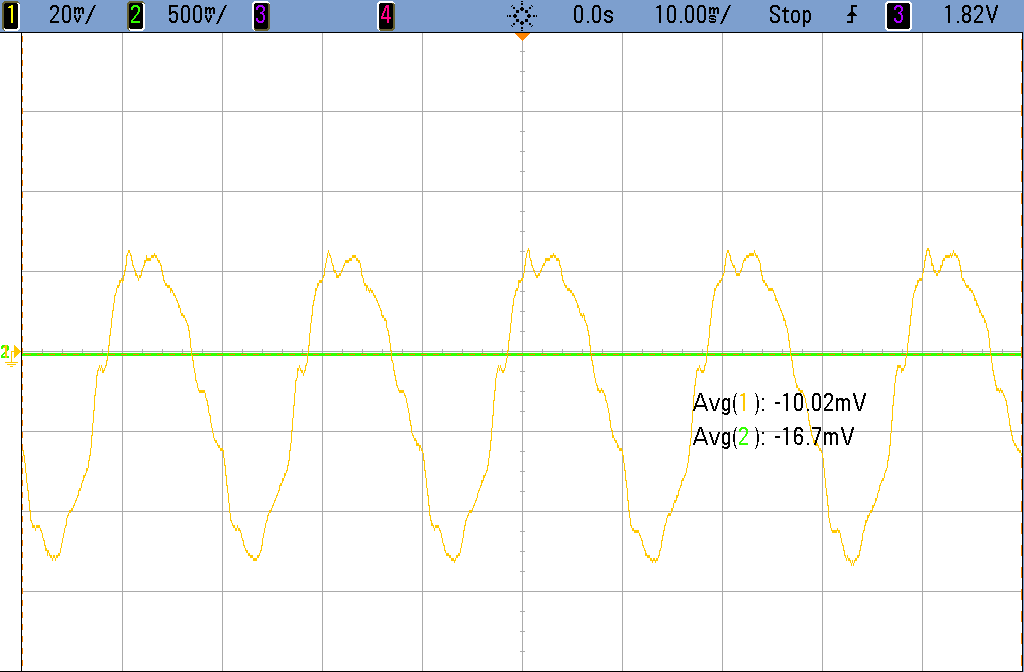
\includegraphics[scale=0.2]{../EJ5/Mediciones/Osciloscopio/CMOS_OR_SOLA/cropped_entrada_al_aire.png} &
        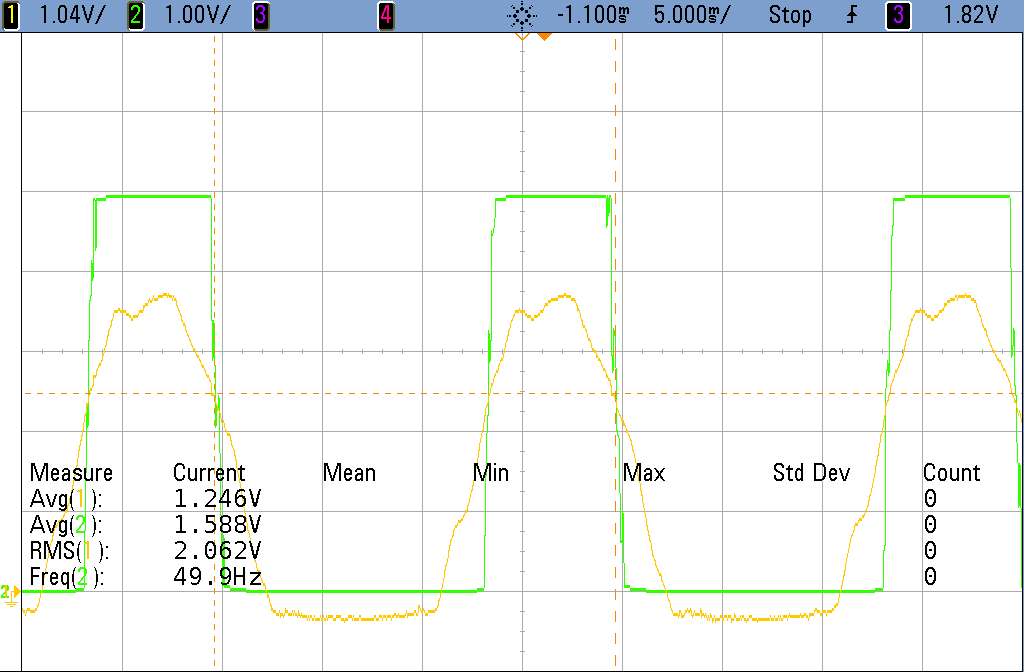
\includegraphics[scale=0.2]{../EJ5/Mediciones/Osciloscopio/CMOS_OR_SOLA/cropped_entrada_ruido.png} 
    \end{tabular}
    \caption{Mediciones para OR tecnolog\'ia CMOS modelo 74HC32}
    \label{fig:cmos_or_al_aire}
\end{figure}

\begin{figure}[H]
    \centering
        \begin{tabular}{c c}
            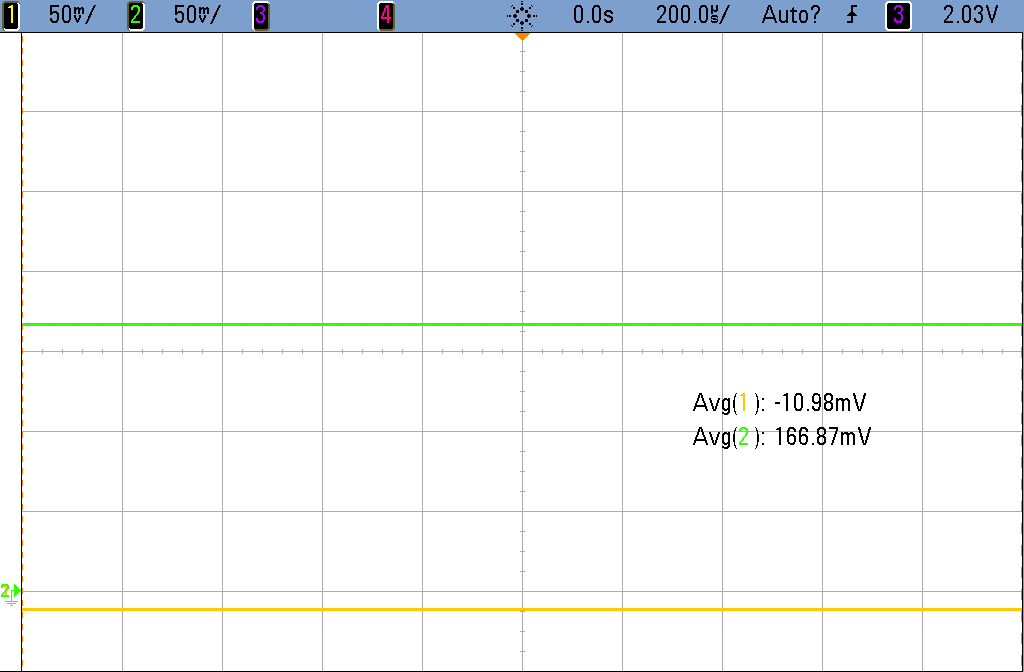
\includegraphics[scale=0.2]{../EJ5/Mediciones/Osciloscopio/TTL_AND_SOLA/cropped_entrada_estado_bajo.png} & 
            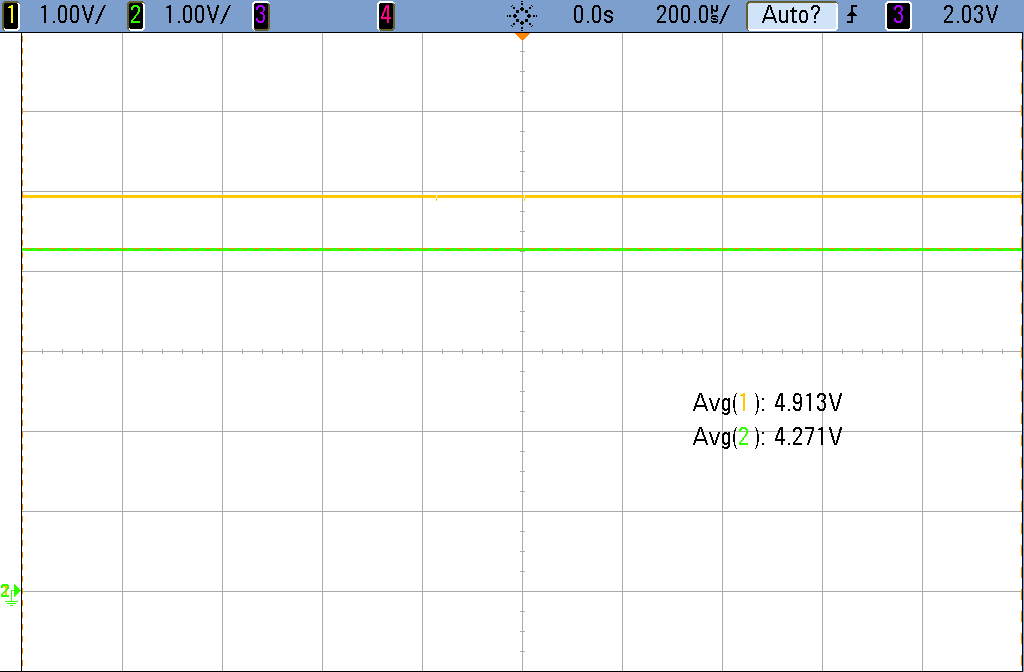
\includegraphics[scale=0.2]{../EJ5/Mediciones/Osciloscopio/TTL_AND_SOLA/cropped_entrada_estado_alto.png} \\ 
            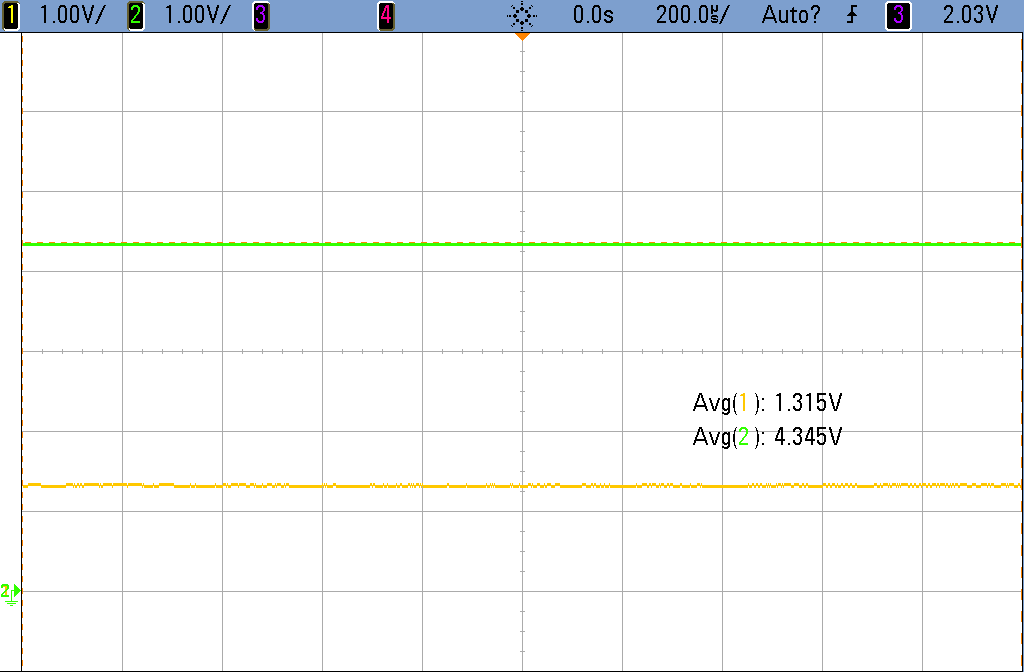
\includegraphics[scale=0.2]{../EJ5/Mediciones/Osciloscopio/TTL_AND_SOLA/cropped_entrada_al_aire.png} & 
            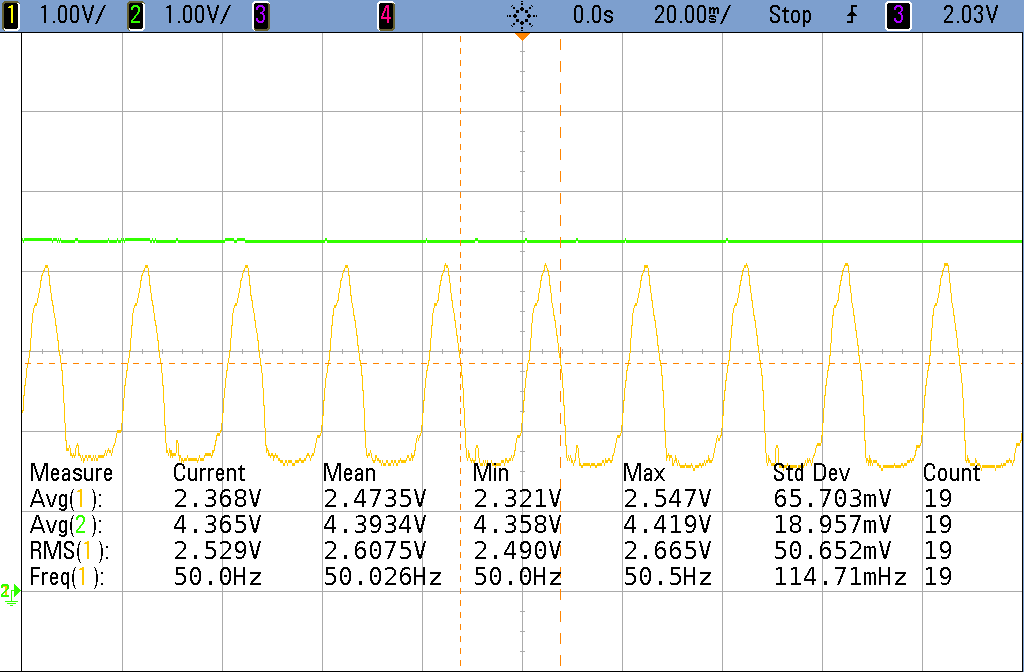
\includegraphics[scale=0.2]{../EJ5/Mediciones/Osciloscopio/TTL_AND_SOLA/cropped_entrada_ruido_frecuencia.png}  
        \end{tabular}
    \caption{Mediciones para AND tecnolog\'ia TTL modelo 74LS08}
    \label{fig:ttl_and_al_aire}
\end{figure}

\subsubsection{An\'alisis de resultados}
En primer lugar, se puede observar que para cada tecnolog\'ia los estados alto y bajo tienen diferente nivel de tensi\'on, lo cual
era esperado a partir de los datos provistos por el fabricante denominados como $V_{OH}$ y $V_{OL}$.

Luego, en principio cuando la entrada se encuentra al aire se puede observar una mayor inmunidad de la tecnolog\'ia TTL frente al ruido,
dado que su valor si bien es indefinido, se mantiene casi constante $V_{IN} \approx 1.315V$, y dado que $V_{IL} = 0.8V < 1.315V < 2V = V_{IH}$ esto indica que
tal nivel se encuentra en donde no est\'a asegurado el comportamiento de la compuerta y por ello la salida tiene tal resultado. Por otro lado, para la entrada al aire,
se puede observar que en la compuerta CMOS hay una oscilaci\'on de la entrada con valor acotados que no producen un cambio sobre la salida.
Esta diferencia entre tecnolog\'ias con una entrada al aire es consecuencia directa de las caracter\'isticas f\'isicas de los transistores MOS, en los cuales la aislaci\'on el\'ectrica
del Gate produce una impedancia de entrada muy elevada para la cual una fuente de ruido de corriente puede producir variaciones de tensi\'on apreciables. Esto \'ultimo puede verse de forma m\'as notoria
cuando se apoya la mano sobre los contactos, ante lo cual el ruido aumenta y la compuerta CMOS recibe una entrada significativa que produce cambios de estado que dan lugar a una oscilaci\'on de la salida,
mientras que en el caso de TTL la se\~nal de ruido no produce un cambio significativo sobre la salida.

Por \'ultimo, es importante aclarar que no es arbitrario que la frecuencia de oscilaci\'on sea aproximadamente $50Hz$, dado que es el ruido de la l\'inea el\'ectrica el que se ve introducido al circuito.

\begin{figure}[H]
    \centering
    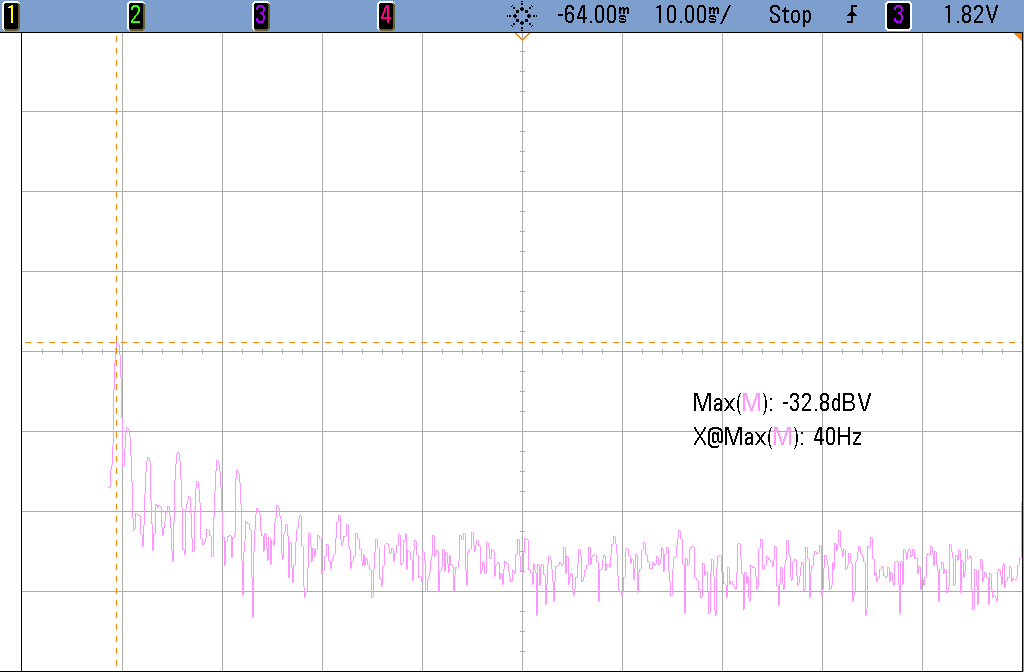
\includegraphics[scale=0.3]{../EJ5/Mediciones/Osciloscopio/CMOS_OR_SOLA/cropped_fft_ruido_contacto.png}
    \caption{FFT aplicada sobre la se\~nal de entrada con la mano apoyada}
    \label{fig:fft_mediciones}
\end{figure}

\subsection{Conexi\'on TTL y CMOS}

\subsubsection{Descripci\'on general}
En la Fig. \ref{fig:ttl_cmos_connected} se ilustra el esquema general del circuito a analizar en esta parte, en la cual el objetivo es analizar el comportamiento
del circuito resultante, partiendo de la base donde la salida ser\'a igual a la entrada aplicando axiomas del algebra booleana.

Se parte de la hip\'otesis de que este circuito podr\'ia presentar un comportamiento alejado del esperado, dado que las tensiones de la tecnolog\'ia TTL y CMOS no son completamente compatibles,
puesto que seg\'un los datos provistos por el fabricante, la TTL entrega una tensi\'on m\'inima de estado alto en $V_{OH} = 2.7V$ mientras que la entrada m\'inima detectada como un estado alto para
CMOS es $V_{IH} = 3.15V$. Para los escenarios del rango intermedio, el circuito se comportar\'a de manera indeterminada.

Se propone realizar mediciones con el objetivo de encontrar las condiciones l\'imite para las cuales se alcanza el problema mencionado anteriormente, puesto que se posible que particularmente la 
compuerta empleada caiga dentro del margen donde el funcionamiento es el esperado. Por esto \'ultimo es que se realizar\'an mediciones con valores de continua, con una se\~nal cuadrada de diversas frecuencias,
y cargando con resistencias o capacitores la salida de las compuertas. Estos procesos buscan simular las exigencias de un circuito sobre la compuerta, llev\'andola al l\'imite para observar que del rango garantizado
por el fabricante en el cual deber\'ia funcionar, el resultante menor.


Es importante aclarar que en la interconexi\'on de compuertas l\'ogicas discretas, es de inter\'es analizar si las corrientes de consumo no superan los valores m\'aximos para cada estado
de la compuerta empleada, no obstante no es un inconveniente en el caso de estudio ya que CMOS por su gran impedancia de entrada posee una corriente de p\'erdida muy inferior a la capacidad
m\'axima de la TTL.

\begin{figure}[H]
    \centering
        \includegraphics[scale=0.6]{../EJ5/Recursos/connection.png}
    \caption{Circuito l\'ogico a ensayar}
    \label{fig:ttl_cmos_connected}
\end{figure}

\subsubsection{Resultados}
En las Figs. \ref{fig:circuit_complete_measures} las se\~nales de color amarillo corresponden a las entradas, las verdes a la salida y luego las de color morado
fueron empleadas para ilustrar el estado de la se\~nal entre ambas compuertas. Las figuras est\'an ordenadas de arriba hacia abajo, de izquierda a derecha, en el orden
de la medici\'on para el estado bajo, estado alto, entrada al aire, con una carga resistiva baja, alta y excedida en la salida TTL.

\begin{figure}[H]
    \centering
    \begin{tabular}{c c}
        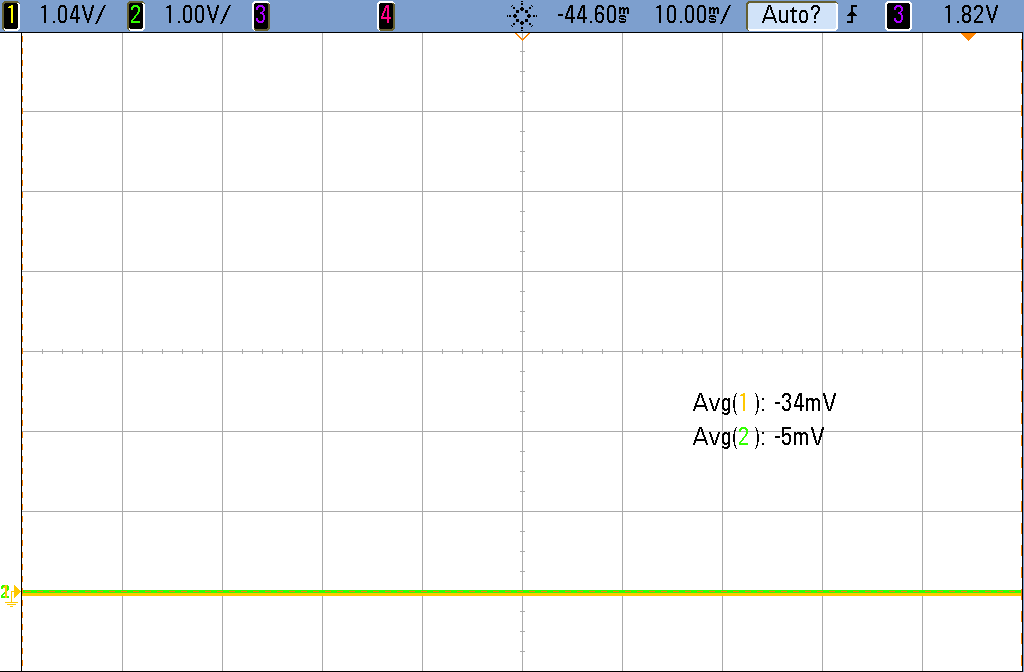
\includegraphics[scale=0.2]{../EJ5/Mediciones/Osciloscopio/CONEXION/cropped_entrada_estado_bajo.png} &
        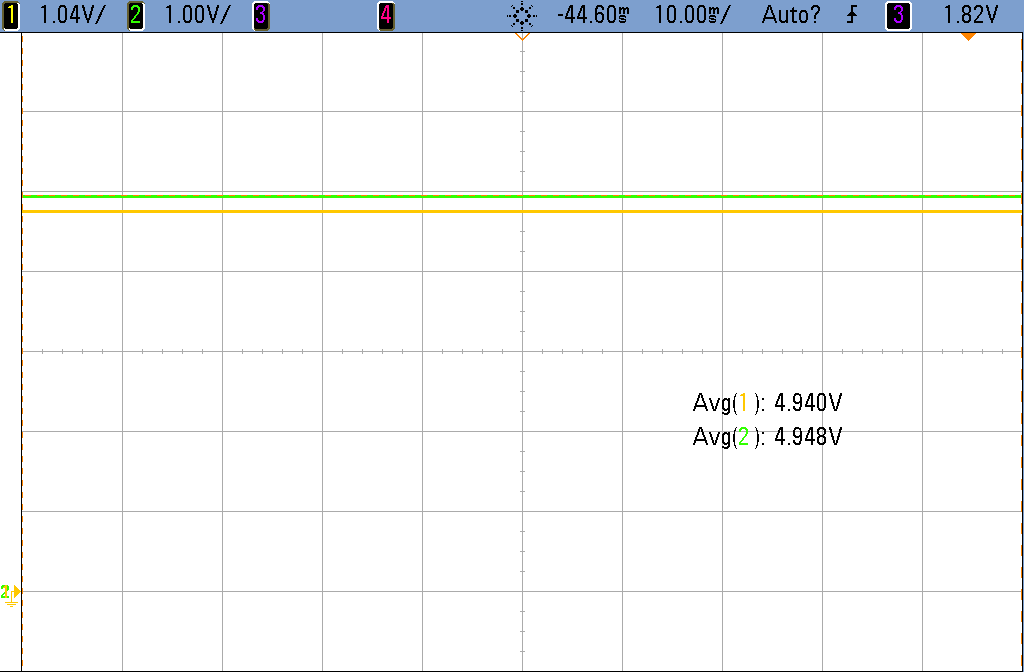
\includegraphics[scale=0.2]{../EJ5/Mediciones/Osciloscopio/CONEXION/cropped_entrada_estado_alto.png} \\
        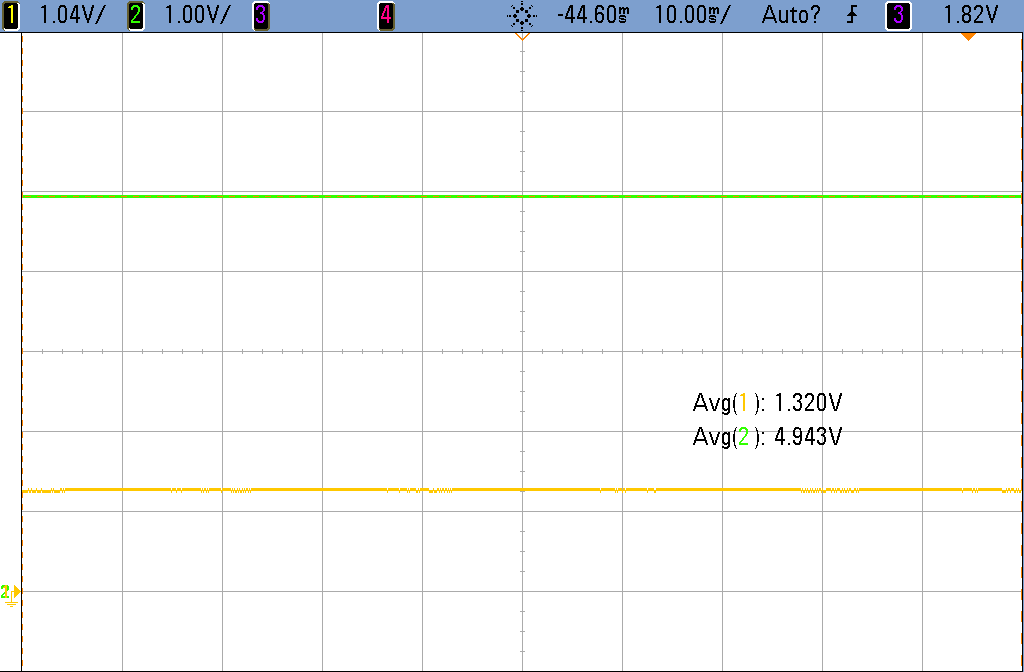
\includegraphics[scale=0.2]{../EJ5/Mediciones/Osciloscopio/CONEXION/cropped_entrada_al_aire.png} &
        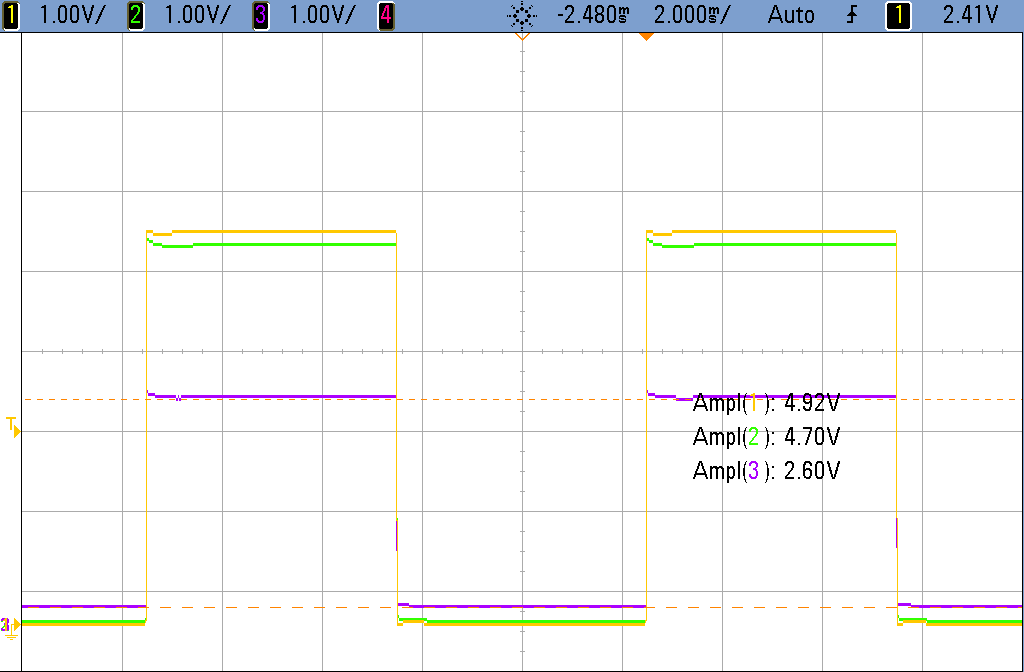
\includegraphics[scale=0.2]{../EJ5/Mediciones/Osciloscopio/CONEXION/cropped_con_carga_baja.png} \\
        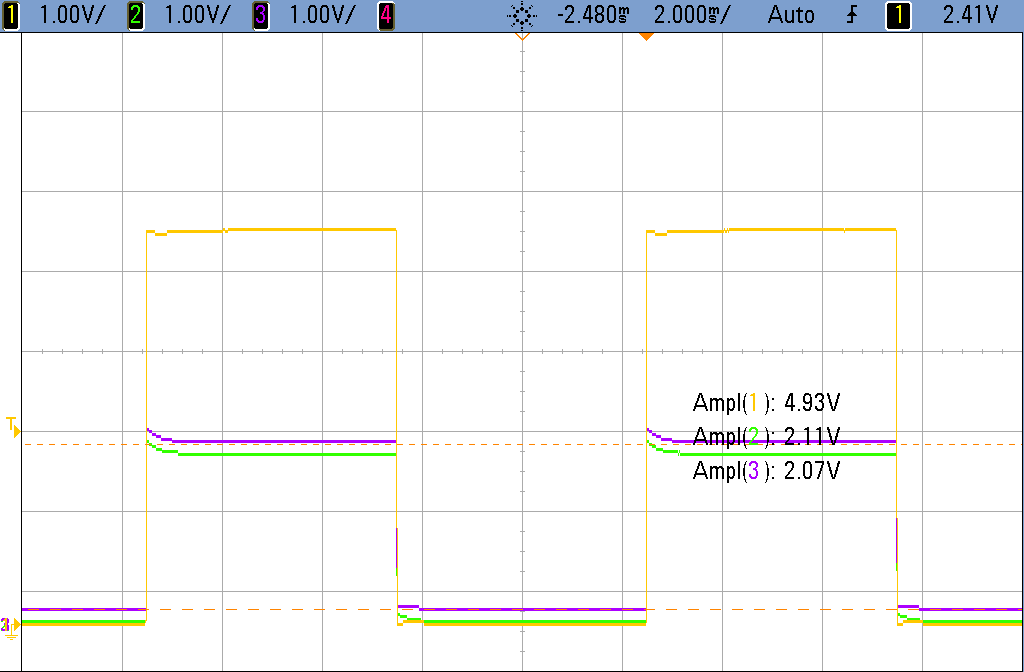
\includegraphics[scale=0.2]{../EJ5/Mediciones/Osciloscopio/CONEXION/cropped_con_carga_alta.png} &
        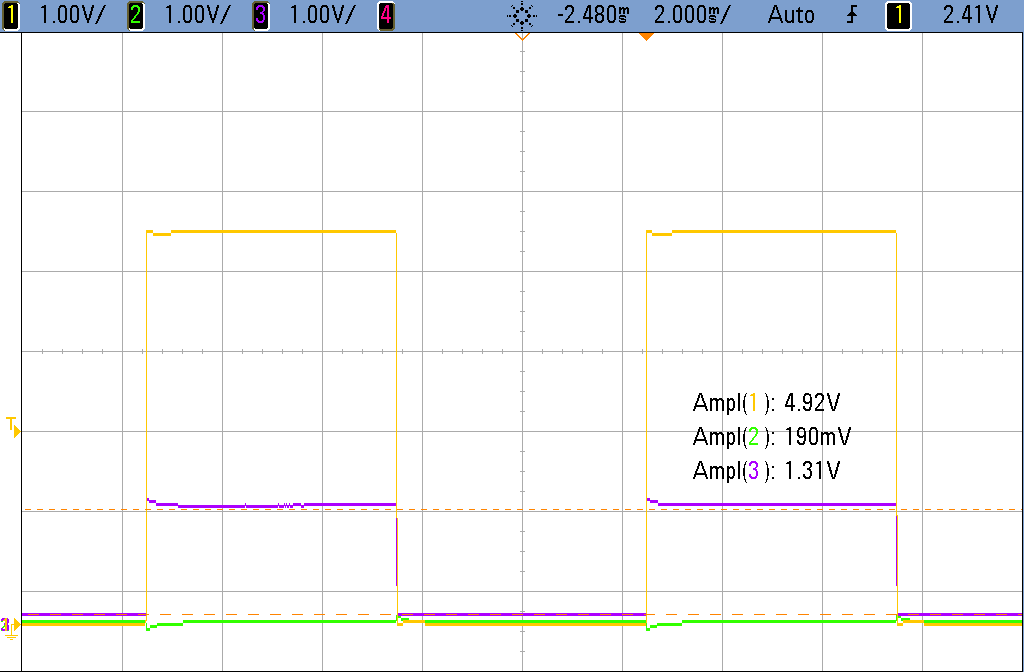
\includegraphics[scale=0.2]{../EJ5/Mediciones/Osciloscopio/CONEXION/cropped_con_carga_excedida.png} \\
    \end{tabular}
    \caption{Mediciones del circuito completo}
    \label{fig:circuit_complete_measures}
\end{figure}

\subsubsection{An\'alisis de resultados}
De los resultados obtenidos puede concluirse que en verdad bajo condiciones donde no se requiere mucho consumo de corriente, entre otras cosas,
la conexi\'on realizada entre una compuerta TTL y una compuerta CMOS es compatible, no obstante, al momento de simular exigencias de corriente por la conexi\'on
de m\'ultiples circuitos, luego los niveles de tensi\'on de la TTL comienzan a bajar cercanos a lo que el fabricante garantiza que sigue siendo un estado alto,
no obstante no es compatible con lo que CMOS reconoce como tal, por lo tanto deja de funcionar como se espera.

Se a\~naden algunas mediciones adicionales que se realizaron en la b\'usqueda de los l\'imites de funcionamiento. Entre estas, se analiz\'o qu\'e suced\'ia
con una se\~nal triangular para ver c\'omo respond\'ian los niveles de tensi\'on de cada tecnolog\'ia, y para altas frecuencias c\'omo afectaban las cargas capacitivas
y los tiempos de propagaci\'on de entrada a salida.

\begin{figure}[H]
    \centering
        \begin{tabular}{c c}
            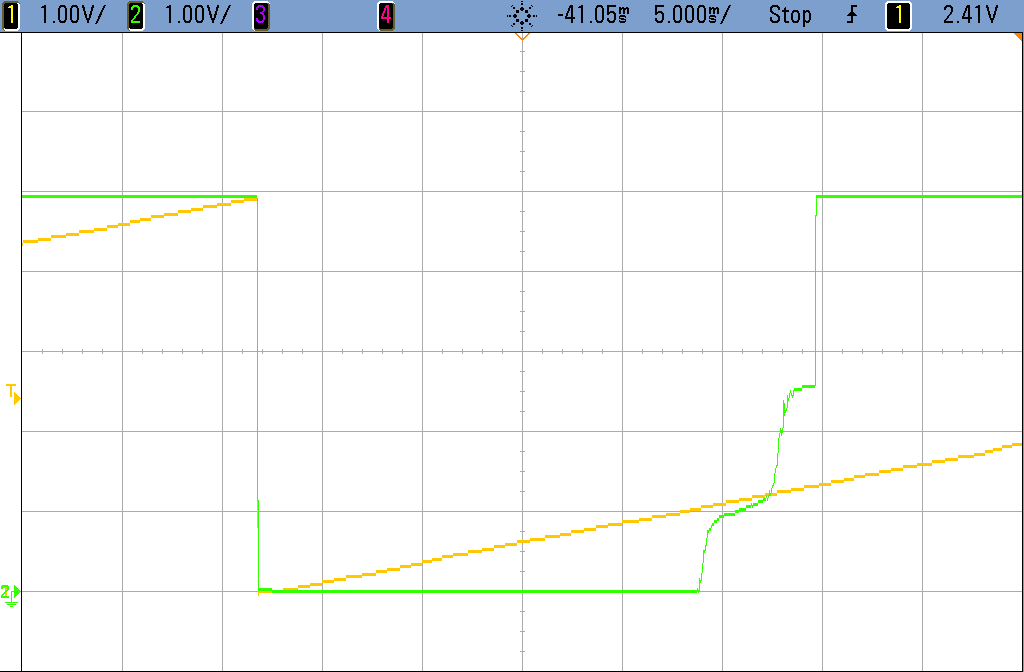
\includegraphics[scale=0.2]{../EJ5/Mediciones/Osciloscopio/CONEXION/cropped_triangular_zoom.png} &
            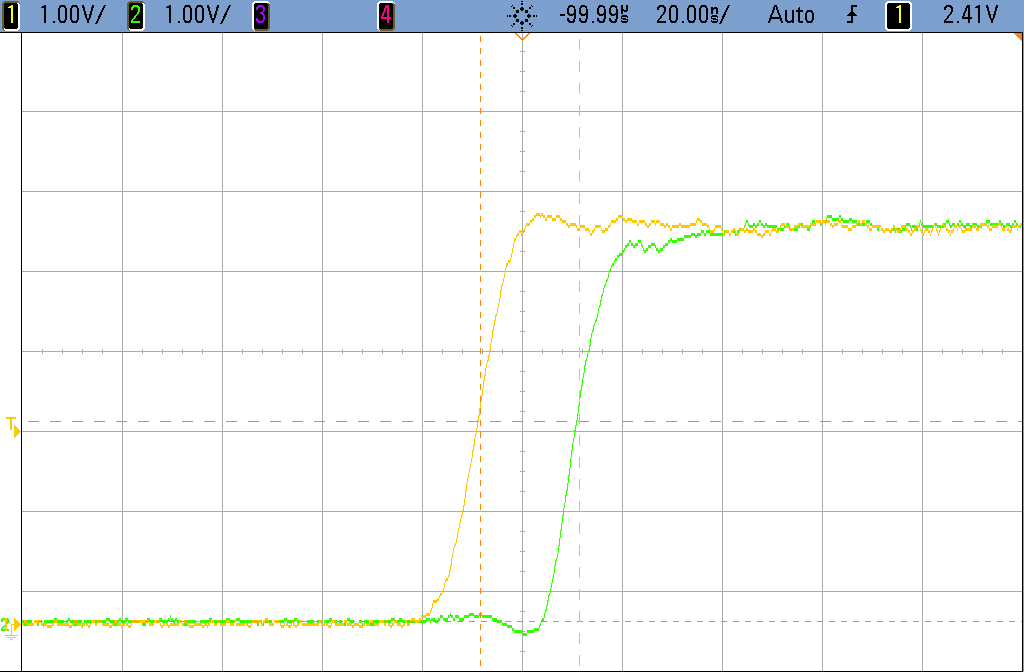
\includegraphics[scale=0.2]{../EJ5/Mediciones/Osciloscopio/CONEXION/cropped_propagacion.png} \\
        \end{tabular}
        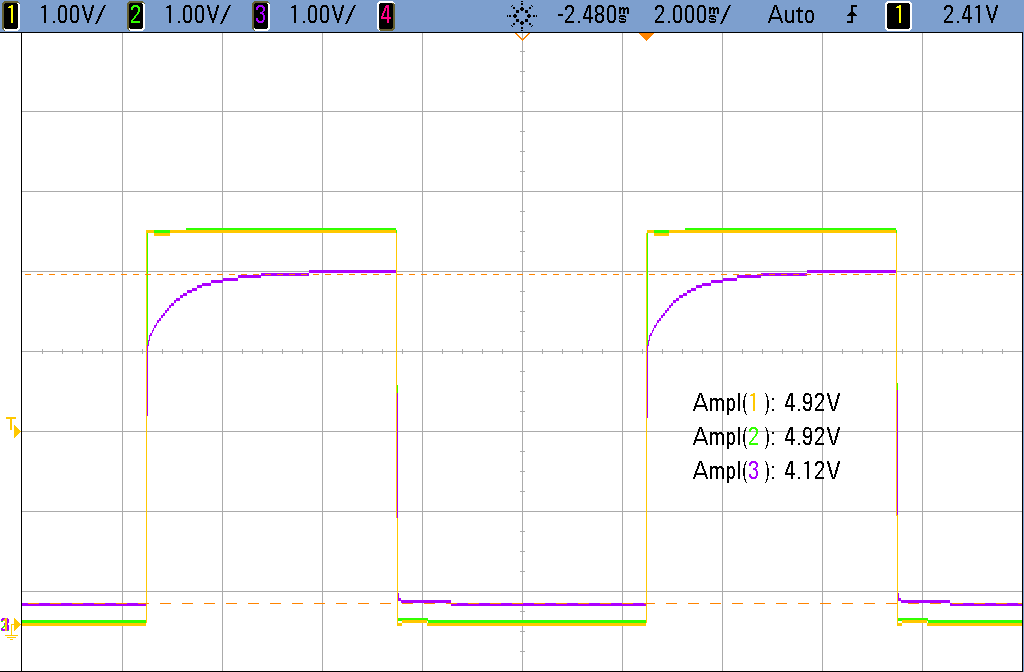
\includegraphics[scale=0.2]{../EJ5/Mediciones/Osciloscopio/CONEXION/cropped_carga_capacitiva.png}
    \caption{Mediciones adicionales}
    \label{fig:additional_measures}
\end{figure}

\subsubsection{Soluciones propuestas}
En las Figs. \ref{fig:circuitos_soluciones} se pueden observar dos circuitos diferentes propuestos como soluci\'on al problema del nivel de tensi\'on para los estados l\'ogicos de una TTL con una CMOS.
Se comparan ambas soluciones dado que la segunda de ellas implementada con un MOSFET es bidireccional, con lo cual la interfaz permite el cambio de nivel en ambos sentidos, pero adem\'as por el hecho de que
permite definir un cambio de nivel de diferentes tensiones. Por el otro lado, la implementaci\'on del circuito con un BJT tipo PNP \'unicamente permite hacer una adaptaci\'on para corregir el nivel de tensi\'on sin cambiarlo,
ya que de otra forma no funcionar\'ia, por ejemplo si se buscara pasar de $3.3V$ a $5V$.

\begin{figure}[H]
    \centering
    \begin{tabular}{c c}
        \includegraphics[scale=0.4]{../EJ5/Recursos/pnp_interface.png} &
        \includegraphics[scale=0.4]{../EJ5/Recursos/mos_interface.png}
    \end{tabular}
    \caption{Circuitos propuestos}
    \label{fig:circuitos_soluciones}
\end{figure}

En las Figs. \ref{fig:resultados_interfaces} la se\~nal amarilla corresponde a la entrada de los circuitos de interfaz, mientras que la morada
corresponde a la salida de los mismos. En la izquierda se observa el resultado de la interface PNP y en la derecha la de NMOS, se puede deducir claramente
que la implementaci\'on de mejor rendimiento es la MOS ya que logra mejor niveles de tensi\'on para cada estado.

\begin{figure}[H]
    \centering
    \begin{tabular}{c c}
        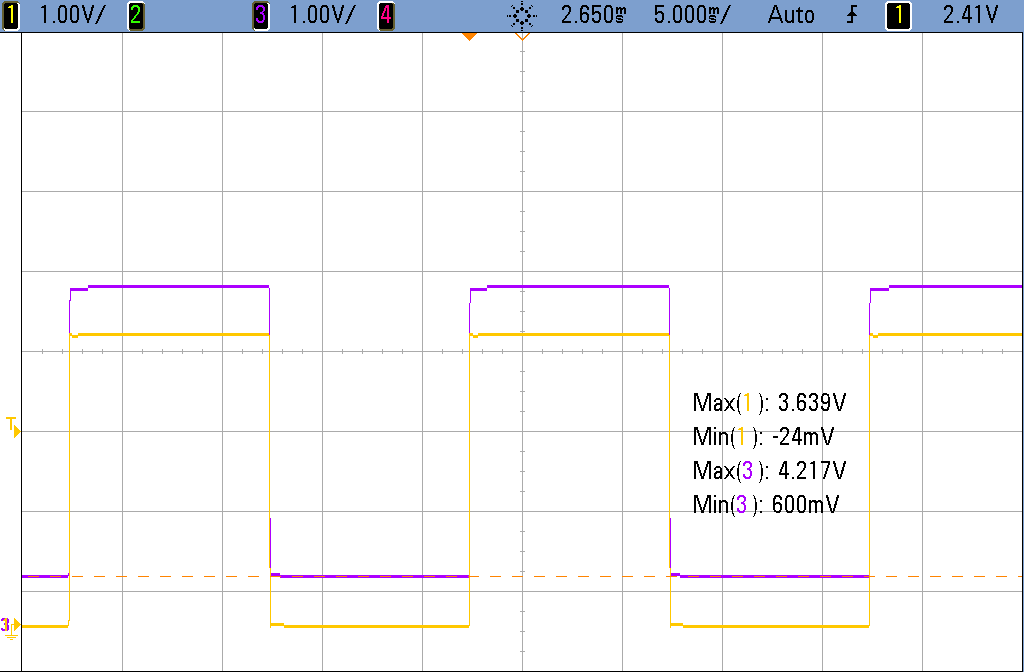
\includegraphics[scale=0.2]{../EJ5/Mediciones/Osciloscopio/LEVEL_SHIFTER/cropped_bjt.png} &
        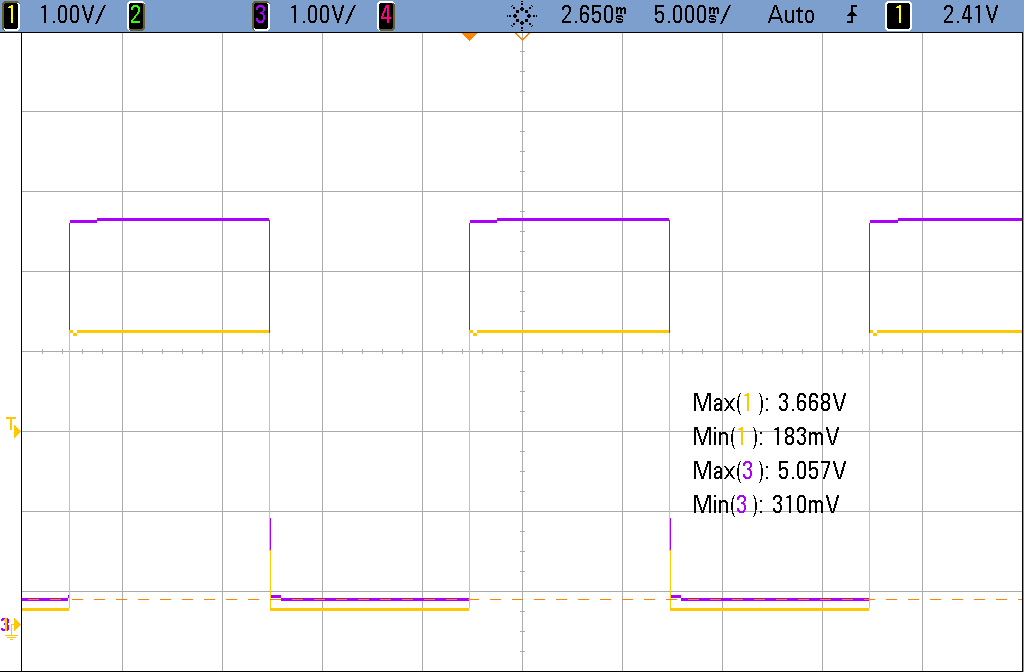
\includegraphics[scale=0.2]{../EJ5/Mediciones/Osciloscopio/LEVEL_SHIFTER/cropped_mos.png} 
    \end{tabular}
    \caption{Resultados de los circuitos implementados ante una se\~nal cuadrada con valores arbitrarios}
    \label{fig:resultados_interfaces}
\end{figure}
